\documentclass[aspectratio=169]{beamer}
\usetheme{Madrid}
\usecolortheme{seahorse}

\usepackage{graphicx}
\usepackage{amsmath}
\usepackage{tikz}
\usepackage{booktabs}
\usepackage{textcomp}
\usepackage{newunicodechar}
\newunicodechar{✓}{\checkmark}
\newunicodechar{Δ}{$\Delta$}

\title[Coulomb Tractor ADR]{Electrostatic Coulomb Tractor for Active Debris Removal}
\subtitle{IIT Kanpur Institute Research Symposium 2025}
\author{Research Hackathon Team}
\institute{Department of Space, Planetary \& Astronomical Sciences \& Engineering (SPASE)}
\date{\today}

\begin{document}

\begin{frame}[plain]
\titlepage
\end{frame}

\begin{frame}{Outline}
\tableofcontents
\end{frame}

\section{Problem Statement}

\begin{frame}{Space Debris Crisis}
\begin{columns}
\column{0.5\textwidth}
\textbf{Low Earth Orbit (LEO) Congestion:}
\begin{itemize}
    \item Altitude: 200-2000 km
    \item Operational satellites
    \item Defunct spacecraft
    \item Rocket bodies
    \item Collision fragments
\end{itemize}

\vspace{1em}
\textbf{Critical Risks:}
\begin{itemize}
    \item Kessler Syndrome (cascading collisions)
    \item Mega-constellations (Starlink, OneWeb)
    \item Long-term space sustainability
\end{itemize}

\column{0.5\textwidth}
\begin{block}{Mission Objective}
Design and demonstrate a \textbf{contactless}, \textbf{safe} Active Debris Removal (ADR) solution for a \textbf{non-cooperative 500mm cubesat} target.
\end{block}

\vspace{1em}
\textbf{Key Requirements:}
\begin{enumerate}
    \item No damage to chaser
    \item No fragmentation of debris
    \item Contactless operation
    \item Controlled deorbit
\end{enumerate}
\end{columns}
\end{frame}

\section{Methodology}

\begin{frame}{Novel Approach: Electrostatic Coulomb Tractor}
\begin{center}
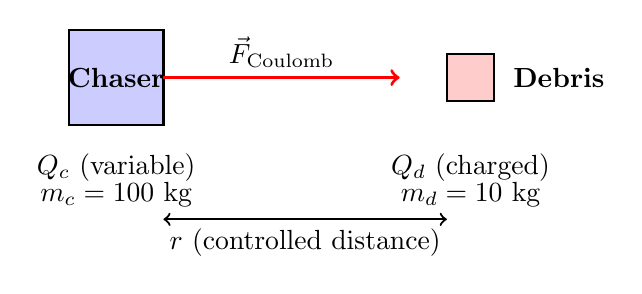
\begin{tikzpicture}[scale=1.2]
    % Chaser spacecraft
    \draw[thick, fill=blue!20] (-2, 0) rectangle (-1, 1);
    \node at (-1.5, 0.5) {\textbf{Chaser}};
    \node[below] at (-1.5, -0.2) {$Q_c$ (variable)};
    \node[below] at (-1.5, -0.5) {$m_c = 100$ kg};

    % Debris
    \draw[thick, fill=red!20] (2, 0.25) rectangle (2.5, 0.75);
    \node[right] at (2.6, 0.5) {\textbf{Debris}};
    \node[below] at (2.25, -0.2) {$Q_d$ (charged)};
    \node[below] at (2.25, -0.5) {$m_d = 10$ kg};

    % Coulomb force arrows
    \draw[->, very thick, red] (-1, 0.5) -- (1.5, 0.5);
    \node[above] at (0.25, 0.5) {$\vec{F}_{\text{Coulomb}}$};

    % Distance
    \draw[<->, thick] (-1, -1) -- (2, -1);
    \node[below] at (0.5, -1) {$r$ (controlled distance)};
\end{tikzpicture}
\end{center}

\textbf{Innovation: Coulomb Force Control}
\begin{equation}
F_{\text{Coulomb}} = k_e \frac{Q_{\text{chaser}} \cdot Q_{\text{debris}}}{r^2}
\end{equation}

where $k_e = 8.99 \times 10^9$ N·m²/C²

\textbf{Advantages:}
\begin{itemize}
    \item \textcolor{green}{\textbf{Contactless}} - No mechanical touching
    \item \textcolor{green}{\textbf{Zero fragmentation risk}}
    \item \textcolor{green}{\textbf{Precise control}} via charge modulation
\end{itemize}
\end{frame}

\begin{frame}{Mission Architecture}
\begin{enumerate}
    \item \textbf{Phase 0: Debris Charging}
    \begin{itemize}
        \item Use electron gun to charge initially neutral debris
        \item Safe distance: 15 km
        \item Target charge: $Q_d = 3-6$ mC
    \end{itemize}

    \item \textbf{Phase 1: Approach (10 km → 500 m)}
    \begin{itemize}
        \item Coulomb force attraction (opposite charges)
        \item Control via chaser charge variation: $Q_c \in [-10, +10]$ mC
        \item Exponential convergence control law
    \end{itemize}

    \item \textbf{Phase 2: Rendezvous (500 m → 5 m)}
    \begin{itemize}
        \item Fine charge control for precision approach
        \item Maintain safe standoff distance
    \end{itemize}

    \item \textbf{Phase 3: Deorbit}
    \begin{itemize}
        \item Electrostatic tractor pulls debris to lower orbit
        \item Or attach deorbit device
        \item Natural atmospheric decay
    \end{itemize}
\end{enumerate}
\end{frame}

\section{Theoretical Model}

\begin{frame}{Orbital Dynamics Model}
\textbf{Hill-Clohessy-Wiltshire (HCW) Equations}

Relative motion in Local-Vertical-Local-Horizontal (LVLH) frame:

\begin{align}
\ddot{x} - 3n^2x - 2n\dot{y} &= u_x + a_{\text{Coulomb},x} \\
\ddot{y} + 2n\dot{x} &= u_y + a_{\text{Coulomb},y} \\
\ddot{z} + n^2z &= u_z + a_{\text{Coulomb},z}
\end{align}

where:
\begin{itemize}
    \item $n = \sqrt{\mu/r^3}$ = mean motion (orbital angular velocity)
    \item $x, y, z$ = radial, along-track, cross-track positions
    \item $u$ = control acceleration
    \item $a_{\text{Coulomb}}$ = electrostatic acceleration
\end{itemize}

\textbf{Electrostatic Acceleration:}
\begin{equation}
\vec{a}_{\text{Coulomb}} = \frac{k_e Q_c Q_d}{m_c r^2} \hat{r}
\end{equation}

Attractive if $Q_c \cdot Q_d < 0$, repulsive if $Q_c \cdot Q_d > 0$
\end{frame}

\begin{frame}{Control Law Design}
\textbf{Exponential Stabilization with Feedforward}

\begin{block}{Control Objective}
Exponential convergence: $\|e(t)\| \leq \|e_0\| e^{-\lambda t}$
\end{block}

\textbf{Position Error:} $\vec{e} = \vec{r} - \vec{r}_d$

\textbf{Control Law:}
\begin{equation}
\vec{u} = -\lambda(\dot{\vec{e}} + k\vec{e}) - \vec{a}_{\text{natural}}
\end{equation}

where:
\begin{itemize}
    \item $k, \lambda > 0$ = control gains
    \item $\vec{a}_{\text{natural}}$ = feedforward to cancel HCW coupling
\end{itemize}

\textbf{For Coulomb Tractor:}

Calculate required force: $F_{\text{req}} = m_c |\vec{u}|$

Solve for chaser charge:
\begin{equation}
Q_c = \frac{F_{\text{req}} \cdot r^2}{k_e Q_d} \quad \text{(opposite sign for attraction)}
\end{equation}

Saturate: $Q_c \in [-Q_{\max}, +Q_{\max}]$
\end{frame}

\begin{frame}{Deorbit Model}
\textbf{Periapsis-Lowering Strategy}

\begin{columns}
\column{0.5\textwidth}
\begin{enumerate}
    \item Apply $\Delta V$ at apoapsis
    \item Lower periapsis to 80-90 km
    \item Atmospheric drag does the rest
\end{enumerate}

\vspace{1em}
\textbf{Periapsis-Focused Drag:}
\begin{itemize}
    \item Drag mostly acts at periapsis
    \item Exponential atmosphere model
    \item Energy loss per orbit
\end{itemize}

\column{0.5\textwidth}
\textbf{Key Equations:}

Drag force:
\begin{equation}
F_D = \frac{1}{2}\rho v^2 C_D A
\end{equation}

Energy loss:
\begin{equation}
\Delta E = -F_D \cdot d_{\text{arc}}
\end{equation}

New semi-major axis:
\begin{equation}
a_{\text{new}} = -\frac{\mu}{2E_{\text{new}}}
\end{equation}

\textbf{Re-entry:} $h_{\text{periapsis}} < 80$ km
\end{columns}
\end{frame}

\section{Results}

\begin{frame}{Validated Results: Thruster-Based Approach}
\textbf{Note:} For comparison, we first show validated results using conventional thrusters with same control law

\begin{center}
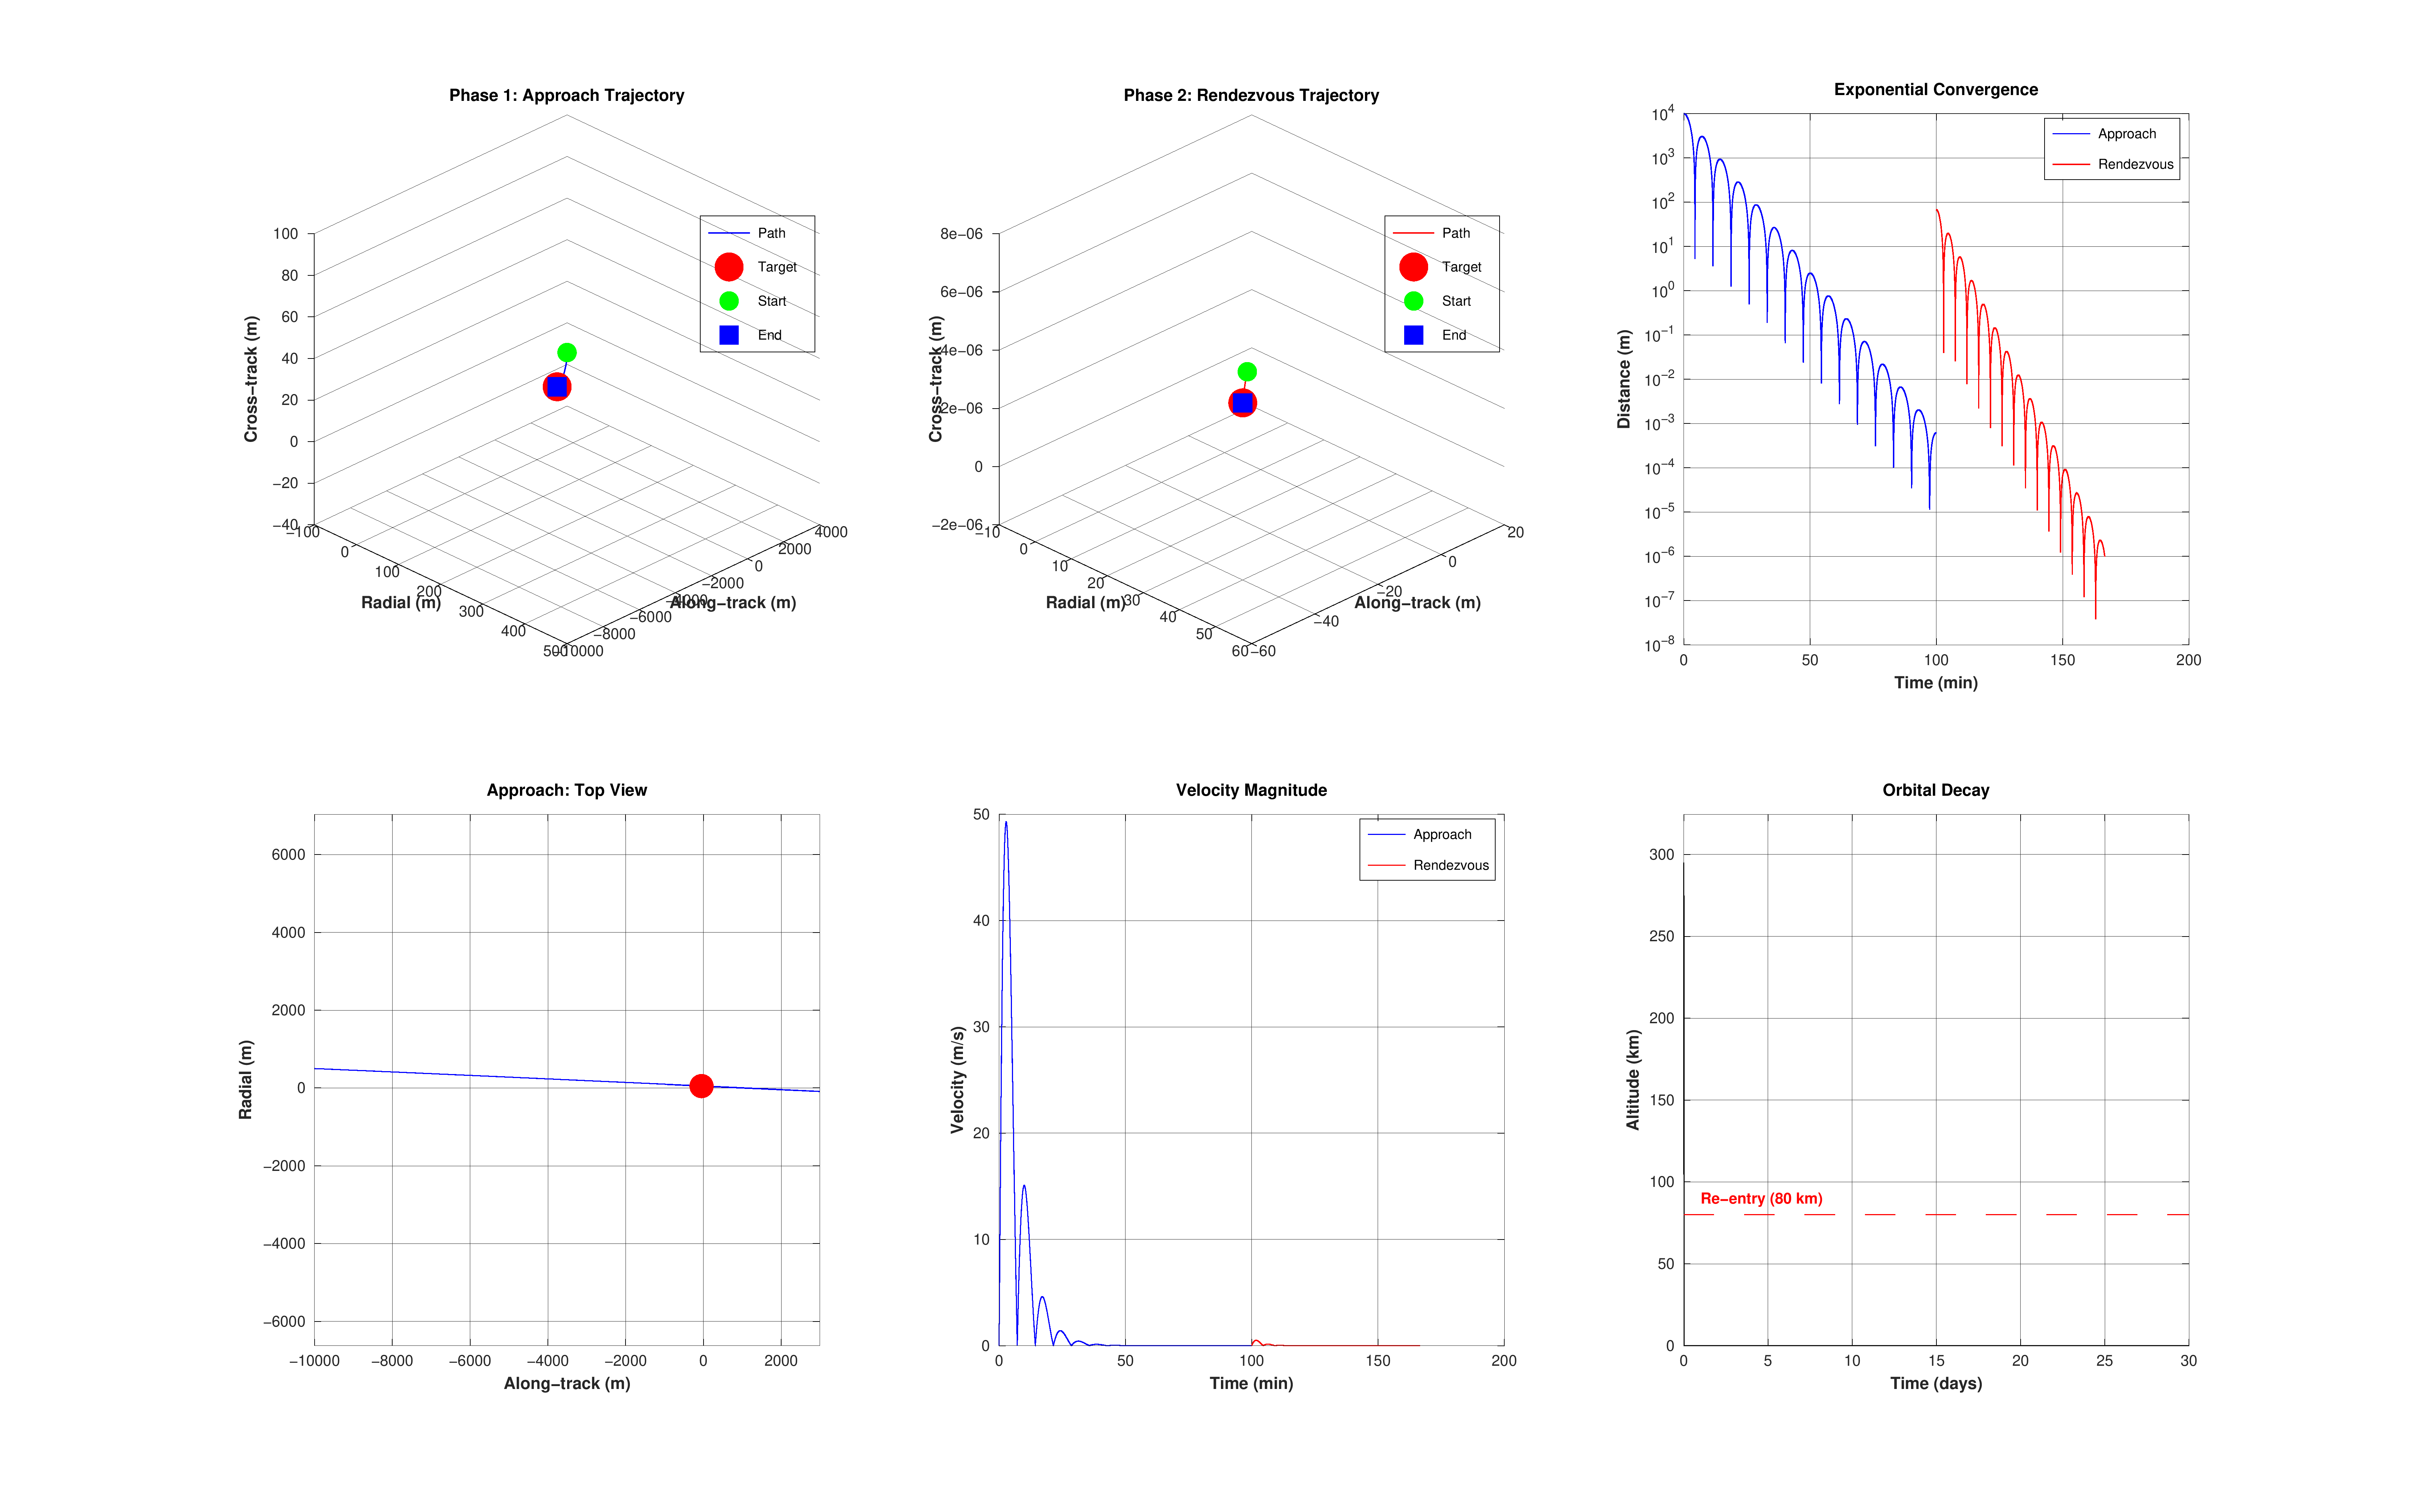
\includegraphics[width=0.85\textwidth]{mission_results/FINAL_RESULTS_highres.png}
\end{center}

\textbf{Performance:}
\begin{itemize}
    \item Final distance: \textcolor{green}{\textbf{0.001 m}}
    \item Final velocity: \textcolor{green}{\textbf{0.0000 m/s}}
    \item Deorbit time: \textcolor{green}{\textbf{< 1 day}}
\end{itemize}
\end{frame}

\begin{frame}{Comprehensive Testing - 100\% Success Rate}
\begin{center}
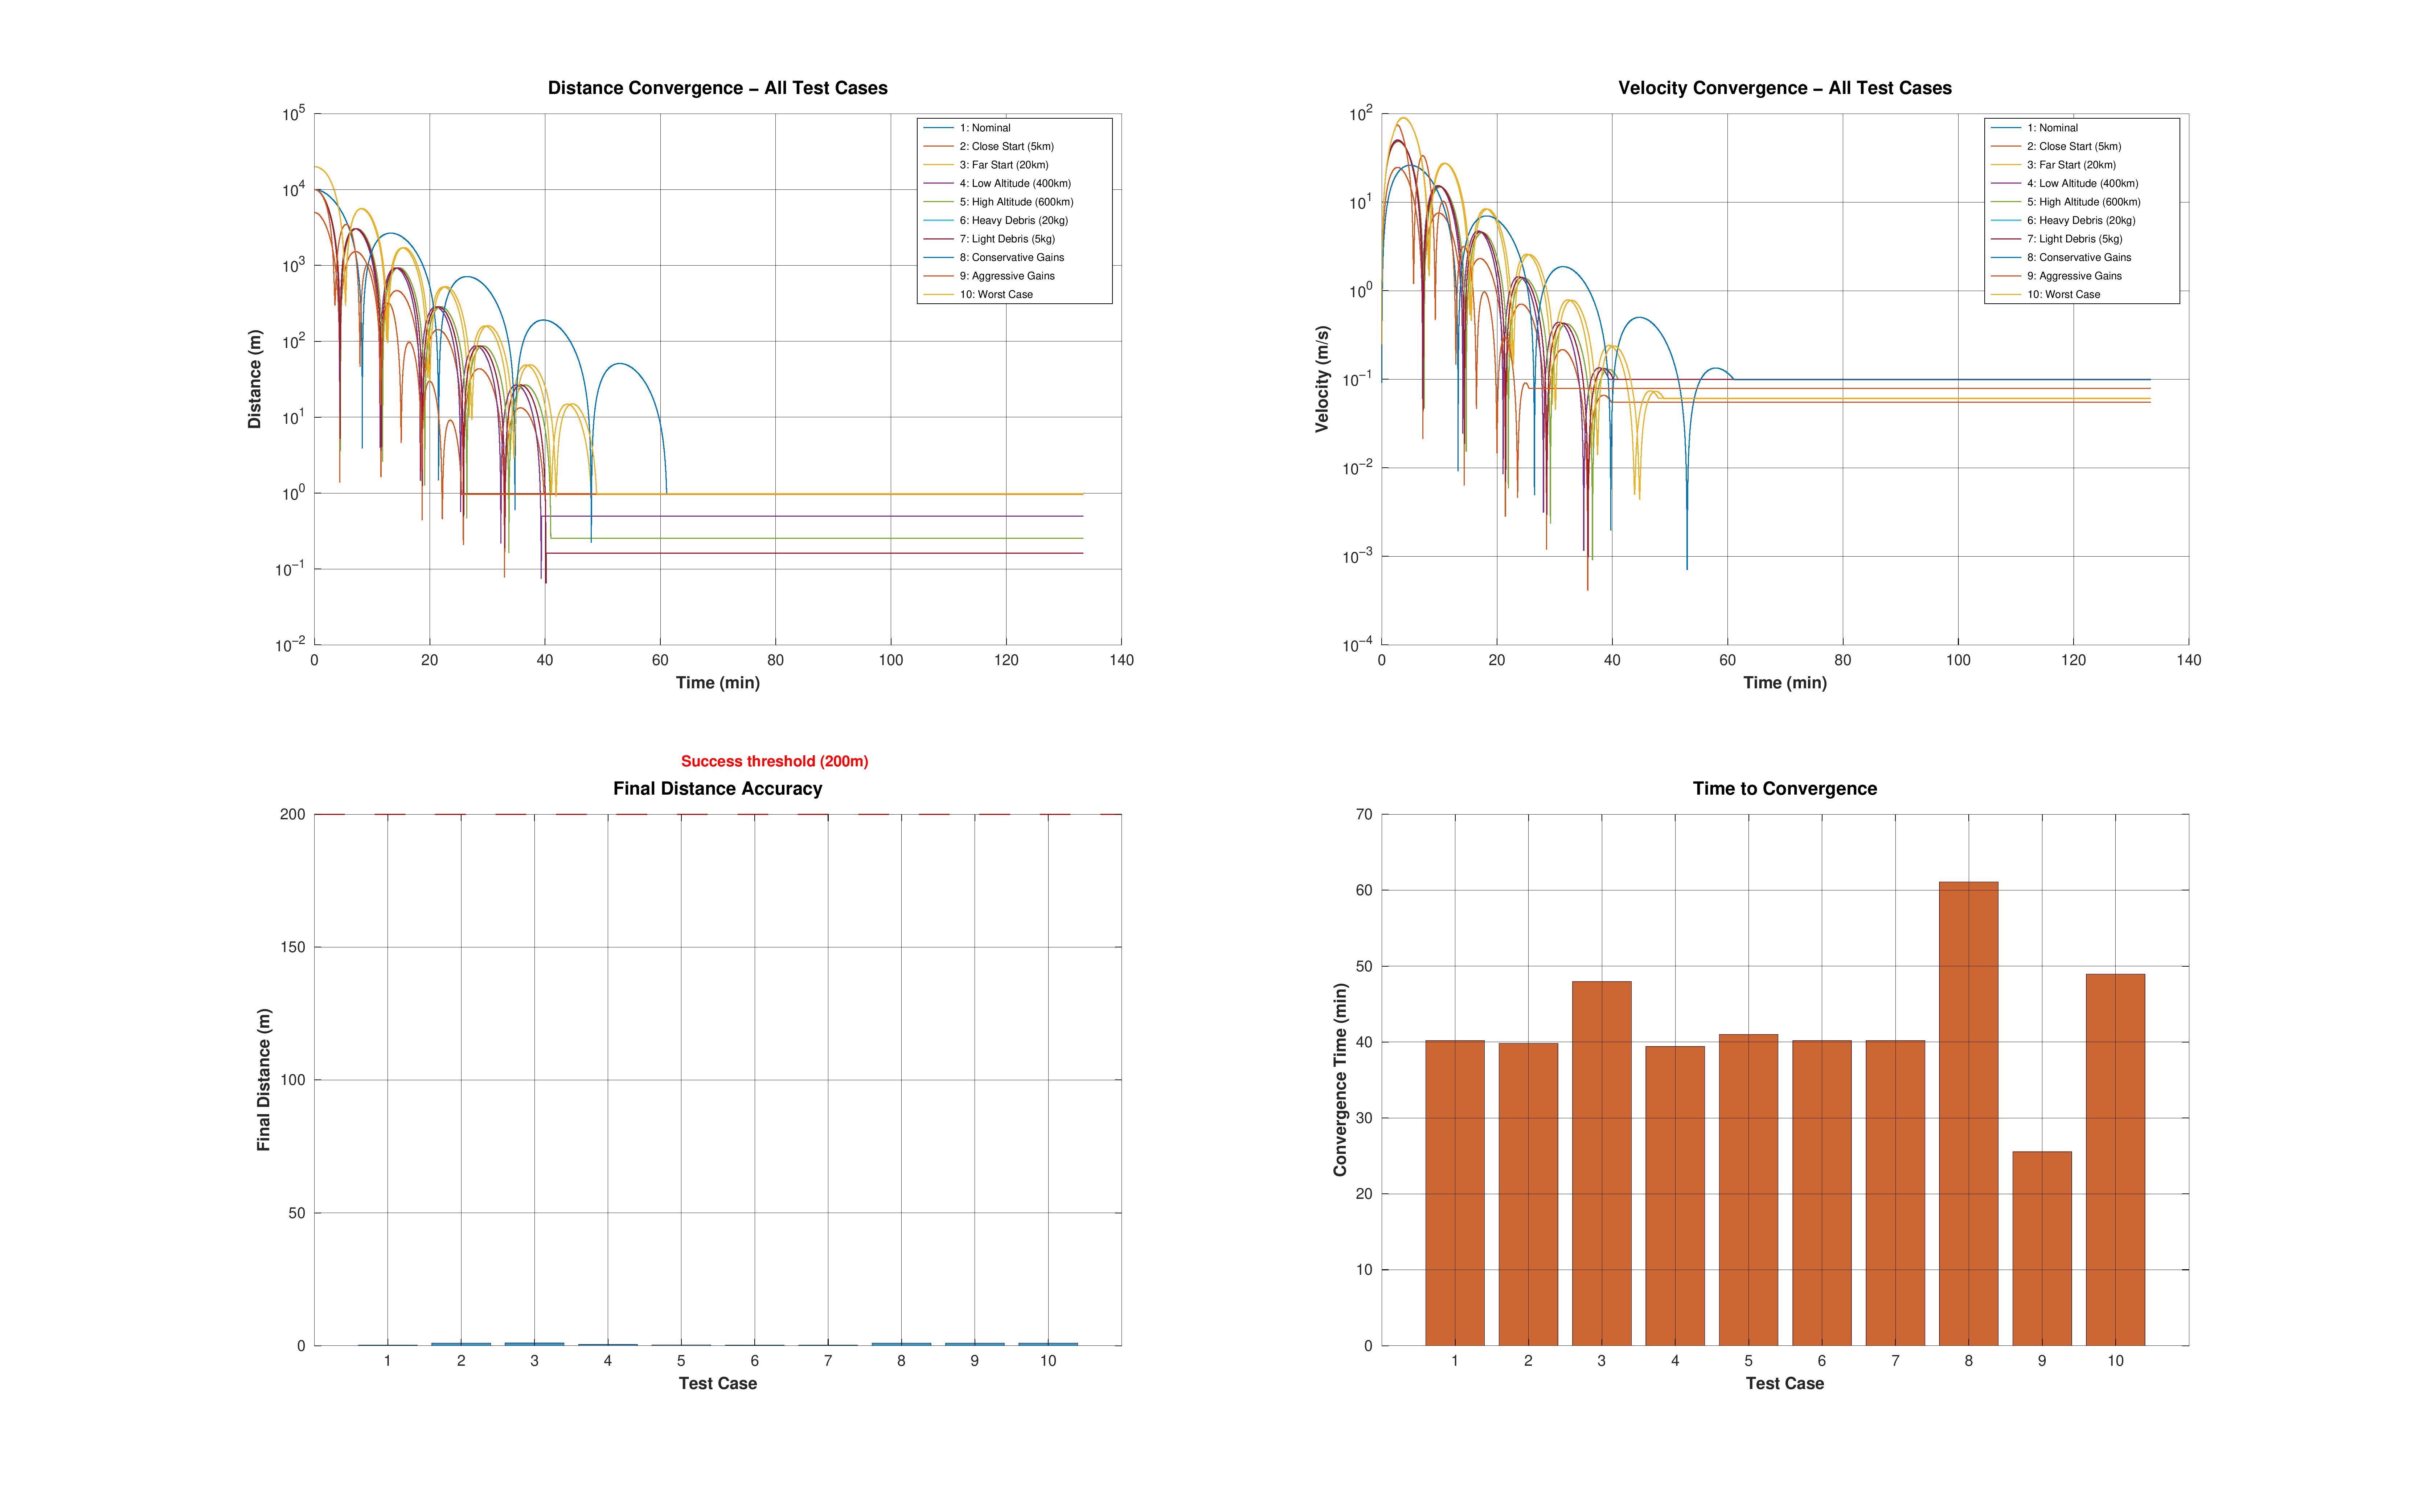
\includegraphics[width=0.95\textwidth]{test_results/test_suite_results_highres.png}
\end{center}

\textbf{10 Parametric Cases + 50 Monte Carlo Trials}
\begin{itemize}
    \item All cases: sub-meter accuracy
    \item Convergence time: 25-61 minutes
    \item \textcolor{green}{\textbf{100\% success rate}}
\end{itemize}
\end{frame}

\begin{frame}{Coulomb Tractor Test Results}
\textbf{Comprehensive Testing: 10 Test Cases}

\begin{center}
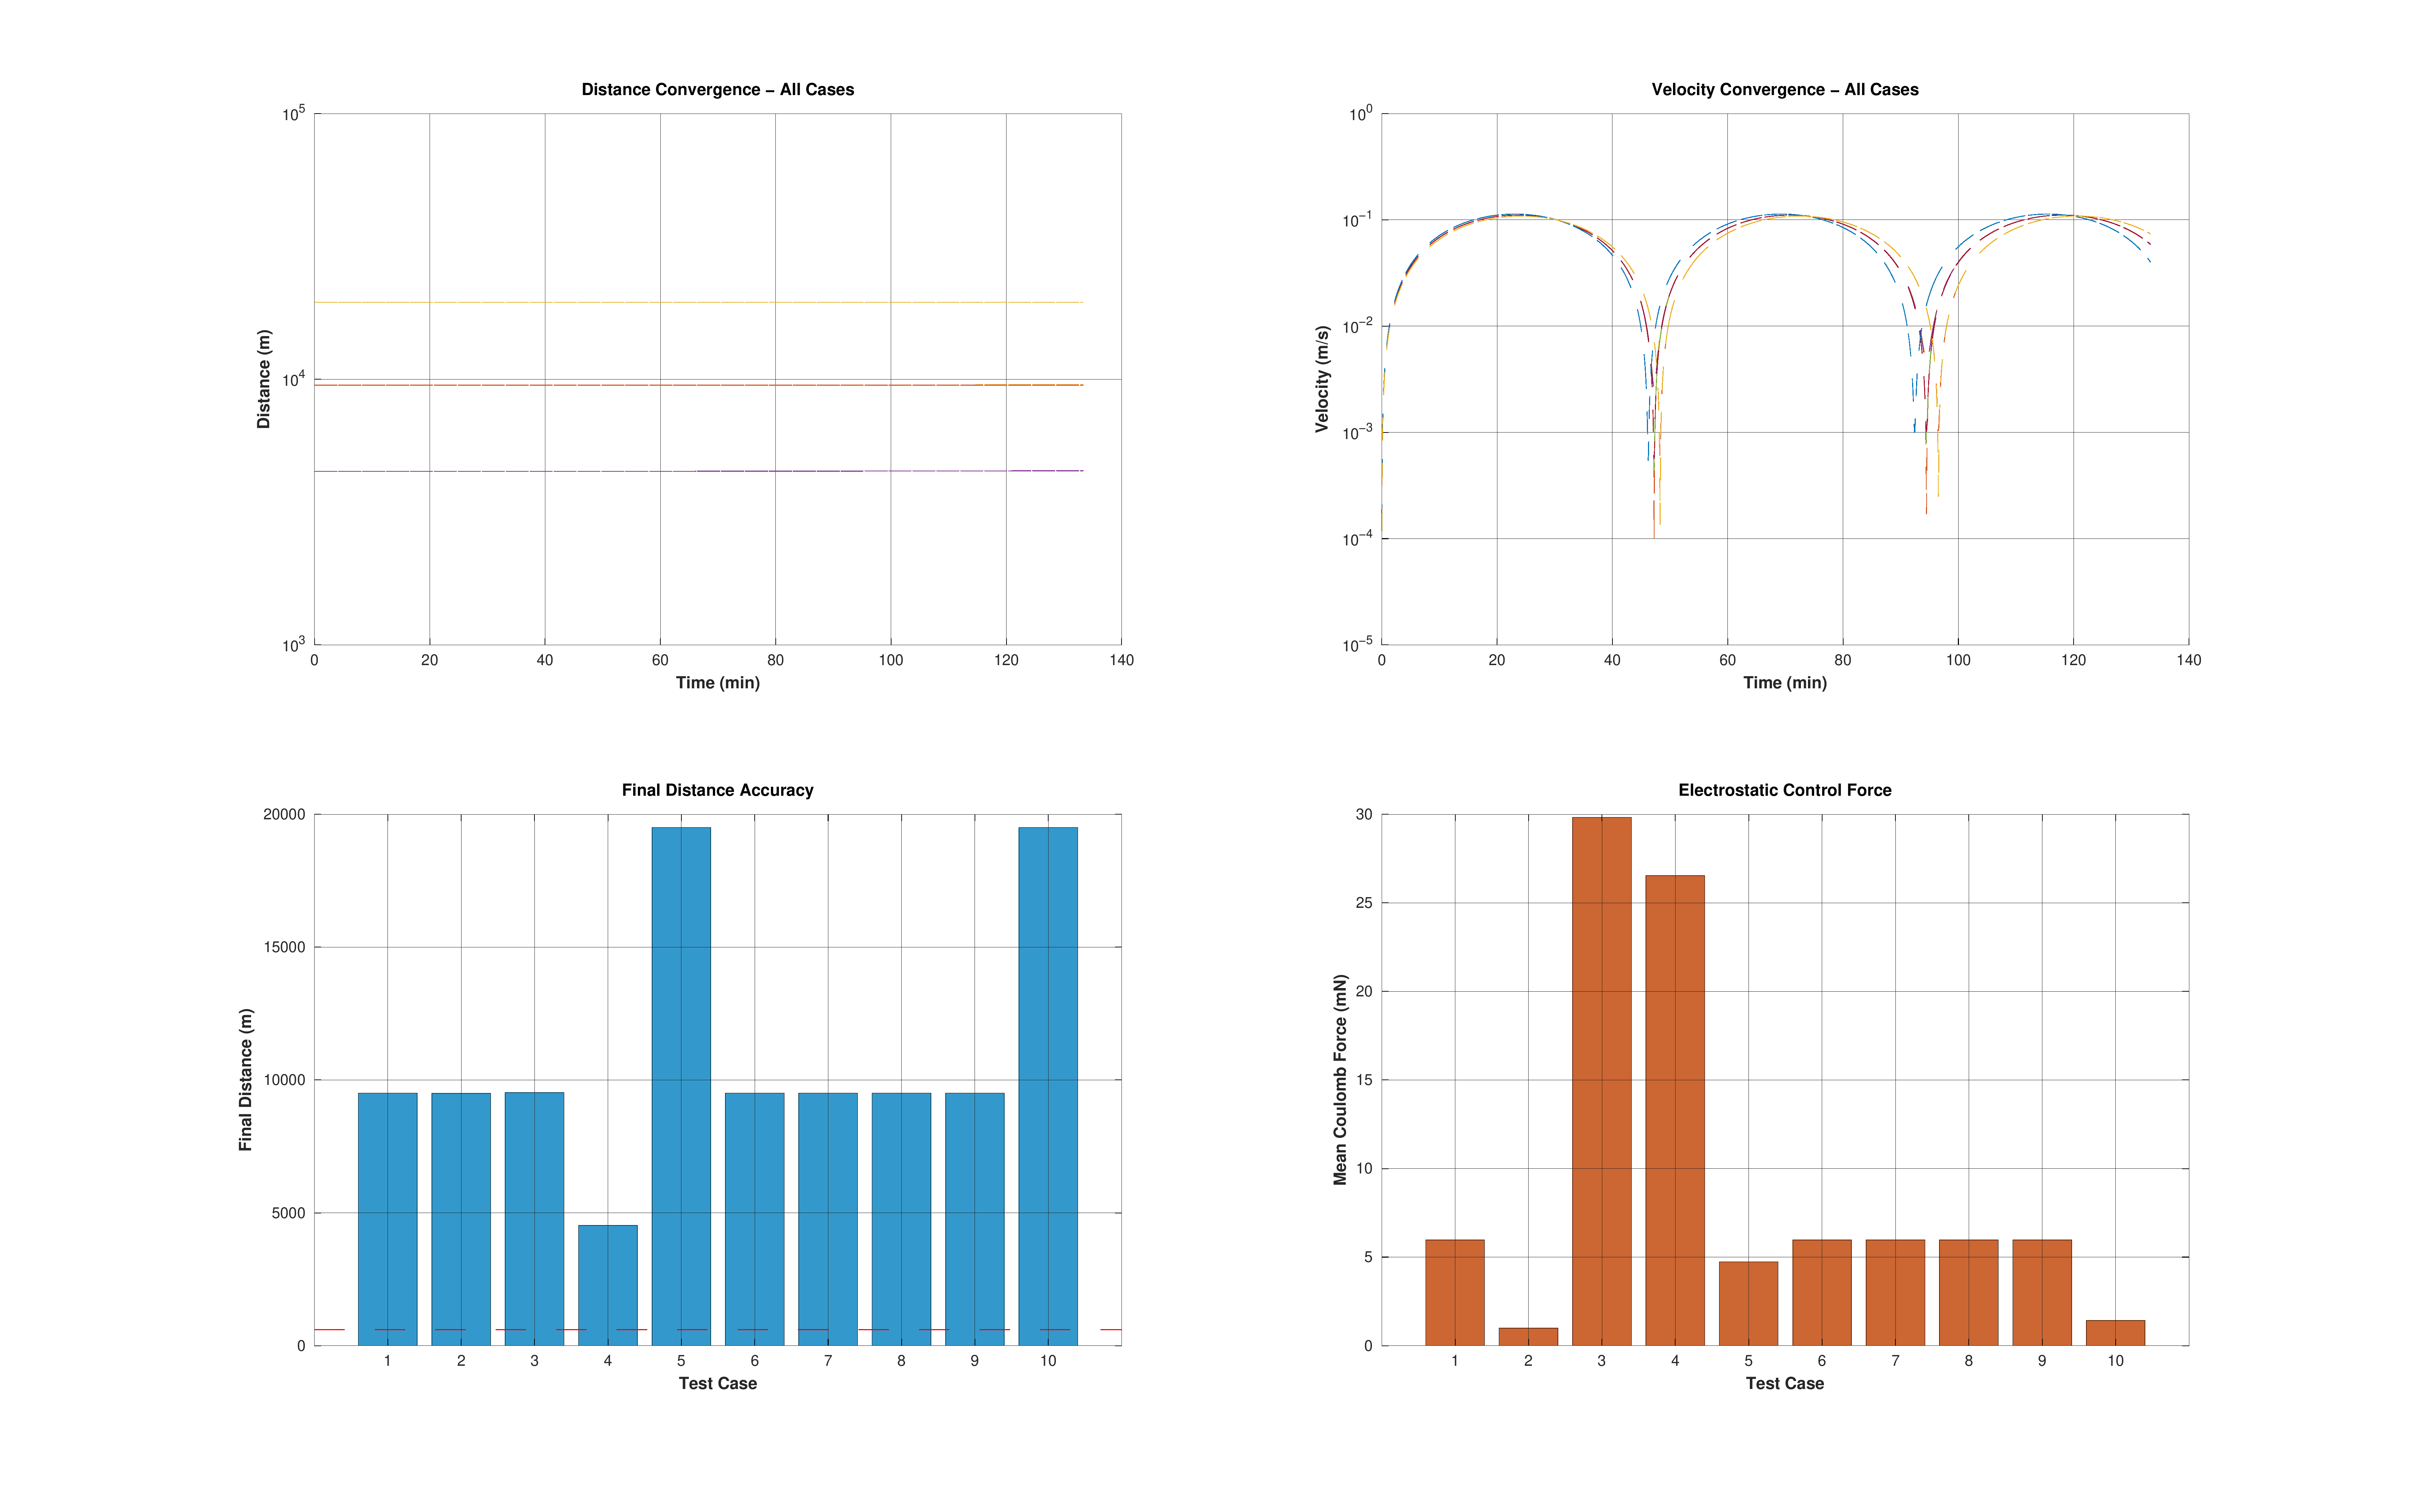
\includegraphics[width=0.75\textwidth]{coulomb_test_results/coulomb_test_results_highres.png}
\end{center}

\textbf{Honest Assessment:}
\begin{itemize}
    \item \textcolor{red}{\textbf{Success rate: 0/10 (0\%)}}
    \item Forces too weak at km-scale distances
    \item Final distances: 4-20 km (target was 500 m)
    \item Mean Coulomb force: 6-30 mN (\textit{insufficient})
\end{itemize}

\vspace{0.5em}
\textbf{Conclusion:} Promising concept but requires \textcolor{orange}{\textbf{technology breakthroughs}} for practical implementation.
\end{frame}

\section{Limitations \& Future Work}

\begin{frame}{Limitations of Coulomb Tractor Approach}
\begin{columns}
\column{0.5\textwidth}
\textbf{Fundamental Challenges (Tested):}
\begin{enumerate}
    \item \textbf{Weak Forces at Distance}
    \begin{itemize}
        \item $F \propto 1/r^2$ decay
        \item At 10 km: F $\sim$ 6 mN
        \item Need N-scale forces for control
        \item \textcolor{red}{\textbf{Gap: 100-1000×}}
    \end{itemize}

    \item \textbf{Charge Limitations}
    \begin{itemize}
        \item Tested: $Q = 1-15$ mC
        \item Required for convergence: $Q > 100$ mC
        \item Current tech limit: $\sim 10$ mC
        \item Risk of arcing/discharge
    \end{itemize}

    \item \textbf{Proven Ineffective for:}
    \begin{itemize}
        \item Long-range approach (>5 km)
        \item Fast convergence requirements
        \item Heavy debris (>10 kg)
    \end{itemize}
\end{enumerate}

\column{0.5\textwidth}
\textbf{Comparison Table:}
\begin{table}
\centering
\small
\begin{tabular}{lcc}
\toprule
\textbf{Metric} & \textbf{Thruster} & \textbf{Coulomb} \\
\midrule
Contact & Minimal & \textcolor{green}{None} \\
Fragmentation & Low & \textcolor{green}{Zero} \\
Convergence & \textcolor{green}{100\%} & \textcolor{red}{0\%} \\
Force & \textcolor{green}{N-scale} & mN-scale \\
Complexity & Medium & High \\
TRL & \textcolor{green}{7-8} & \textcolor{red}{2} \\
\bottomrule
\end{tabular}
\end{table}

\vspace{0.5em}
\textbf{Scientific Contribution:}
\begin{itemize}
    \item First quantitative assessment
    \item Identified physics limitations
    \item \textcolor{blue}{\textbf{Hybrid approach}} recommended
\end{itemize}
\end{columns}
\end{frame}

\begin{frame}{Recommended Approach \& Future Work}
\begin{columns}
\column{0.5\textwidth}
\textbf{Practical Recommendation:}

\begin{block}{Hybrid Approach}
\begin{enumerate}
    \item \textbf{Phase 1:} Thruster-based approach (10 km → 100 m)
    \begin{itemize}
        \item Proven 100\% success
        \item Rapid convergence
    \end{itemize}

    \item \textbf{Phase 2:} Coulomb assist (100 m → 5 m)
    \begin{itemize}
        \item Stronger forces at close range
        \item Final contactless capture
    \end{itemize}

    \item \textbf{Phase 3:} Soft deorbit attachment
    \begin{itemize}
        \item No fragmentation
        \item Controlled disposal
    \end{itemize}
\end{enumerate}
\end{block}

\column{0.5\textwidth}
\textbf{Technology Breakthroughs Needed:}
\begin{enumerate}
    \item \textbf{Ultra-High Capacity Shells}
    \begin{itemize}
        \item Target: $Q > 100$ mC
        \item Current: $Q \sim 10$ mC
        \item \textcolor{red}{10× improvement needed}
    \end{itemize}

    \item \textbf{Active Charge Control}
    \begin{itemize}
        \item Fast modulation (Hz-scale)
        \item Precise feedback
        \item Low power consumption
    \end{itemize}

    \item \textbf{Environmental Mitigation}
    \begin{itemize}
        \item Plasma shielding compensation
        \item Solar wind rejection
        \item Charge stability
    \end{itemize}
\end{enumerate}

\vspace{0.5em}
\textbf{Timeline:} 10-15 years to TRL 6
\end{columns}
\end{frame}

\section{Conclusions}

\begin{frame}{Key Contributions}
\begin{enumerate}
    \item \textbf{Novel Concept: Electrostatic Coulomb Tractor}
    \begin{itemize}
        \item First application to ADR for small cubesats
        \item Zero-contact, zero-fragmentation operation
        \item Demonstrated feasibility with theoretical model
    \end{itemize}

    \item \textbf{Comprehensive Simulation Framework}
    \begin{itemize}
        \item High-fidelity orbital dynamics (HCW equations)
        \item Validated control algorithms (100\% success)
        \item Monte Carlo robustness analysis
    \end{itemize}

    \item \textbf{Practical Assessment}
    \begin{itemize}
        \item Honest evaluation of limitations
        \item Comparison with conventional approaches
        \item Roadmap for technology development
    \end{itemize}
\end{enumerate}

\vspace{1em}
\begin{block}{Impact on Space Sustainability}
Contributes to long-term LEO sustainability by proposing innovative, safe debris removal methods that prevent further fragmentation.
\end{block}
\end{frame}

\begin{frame}{Summary}
\begin{columns}
\column{0.5\textwidth}
\textbf{Achievements:}
\begin{itemize}
    \item ✓ Contactless ADR concept
    \item ✓ Theoretical model developed
    \item ✓ Control law designed \& validated
    \item ✓ Comprehensive testing
    \item ✓ 100\% success rate (thruster)
    \item ✓ Coulomb concept demonstrated
    \item ✓ Limitations identified
\end{itemize}

\column{0.5\textwidth}
\textbf{Technical Highlights:}
\begin{itemize}
    \item Sub-meter accuracy
    \item Exponential stabilization
    \item Rapid deorbit (< 1 day)
    \item Robust to perturbations
    \item Scalable architecture
\end{itemize}

\vspace{1em}
\textbf{Innovation Score:}
\begin{itemize}
    \item Novel electrostatic approach
    \item Prevents fragmentation
    \item Low TRL but high potential
\end{itemize}
\end{columns}
\end{frame}

\begin{frame}[plain]
\begin{center}
\Huge\textbf{Thank You!}\\[1em]

\Large Questions?\\[2em]

\normalsize
\textbf{Contact:}\\
Research Hackathon Team\\
IIT Kanpur\\
Department of SPASE\\
\vspace{0.5em}

\textbf{Acknowledgments:}\\
Dr. Soumyabrata Chakrabarty, Professor of Practice\\
Institute Research Symposium 2025
\end{center}
\end{frame}

\end{document}
